\section{Evaluation protocol, source records and adjudication}\label{app:protocol}
This appendix adds descriptive analyses of the released records without changing benchmark units, model answers or five-axis judgments. The 4,104 Task 1, 4,632 Task 2 and 480 Task 3 consolidated rows were checked against the archived per-run prediction files; all Task 2/3 axis values were checked against their judgment files. All 9,216 row comparisons passed. Derived chain indicators equal the product of the five binary axes, and joint indicators equal answer correctness times chain correctness. File-integrity checks passed for the original release manifest. These checks validate artifact consistency, not biological annotation quality or judge reliability.

The five text-only systems use prompts specifying no retrieval or external tools; Biomni uses a tool-augmented setting. Each has four recorded runs. GPT outputs are judged by Claude; the remaining systems are judged by GPT, according to the released protocol. No blinded human agreement estimate is supplied by this revision. A different model family judging an answer does not eliminate evaluator bias. Shared failures across judges or systems are descriptive observations, not an independent validation of a gold mechanism.

The frozen scorer is retained unchanged. Task 3 aggregate results apply the separately disclosed entity-conditional alias: for entities recognized by the released amendment as regulatory RNA (the implementation checks for ``mir'' in the entity string), canonical knockdown is treated as inhibition. This implementation is narrower than an alias for all possible RNA entities. Strict matching retains interpretable noncompliant responses as incorrect, including Claude Task 3 run 2. Reported re-administrations and original captures are documented in the repository. The old aggregate scripts contain paths from the pre-release directory layout; the accompanying revision supplies a separate portable audit entry point and does not rewrite frozen answers or judgments.

\paragraph{Three levels of evidence.} Benchmark inputs define the information supplied to a system; evaluator-only annotations specify the curated mechanism, mediator and experimental contrast; archived responses and five-axis judgments record how the system was evaluated. These levels must be distinguished when interpreting a failure. The public release now includes reference annotations for inspection, but those annotations were withheld from the evaluated text-only systems.
\begin{center}
\begin{tabular}{lrrrrr}
\toprule
Task & Distinct pairs & Units/run & Systems & Runs/system & Records \\
\midrule
1 & 171 & 171 & 6 & 4 & 4,104 \\
2 & 168 & 193 & 6 & 4 & 4,632 \\
3 & 9 & 20 & 6 & 4 & 480 \\
\bottomrule
\end{tabular}
\end{center}
\paragraph{Scope of the added analyses.} This supplement recomputes descriptive summaries from the frozen records and checks their correspondence to archived predictions and judgments. It adds no model runs, training experiments or replacement judgments. Biological interpretation is anchored to the primary experimental sources cited in the module sections. These are regulatory dependency modules rather than TF families defined by sequence homology. Counts of targets, units and repeated judgments are provided separately.

\paragraph{Reliability boundary.} Cross-model scoring avoids direct self-judging but does not establish human agreement. The targeted review records on page~\pageref{app:concentration} identify specific discrepancies rather than assuming that all released judgments are biologically definitive. A reproducible numerical result and a validated biological judgment are different forms of evidence.

\clearpage
\section{Metric definitions and complete pass-rate summaries}\label{app:metrics}
Table~\ref{tab:model_performance} uses answer-only balanced accuracy and macro-F1 for Task 1, but chain-dependent joint metrics for Tasks 2/3. These must not be read as answer-only direction or intervention-type scores. Let $z_{ic}$ indicate membership of unit $i$ in reference class $c$, $p_{ic}$ indicate prediction of that class, and $C_i$ be the five-axis pass indicator. Balanced joint accuracy averages $\sum_i z_{ic}p_{ic}C_i/\sum_i z_{ic}$ equally over reference classes. Task 3 allows a set of accepted intervention labels, so membership refers to the released accepted set after normalization.

For transparency, the published Task 2 joint F1 implementation counts $TP_c=\sum_i z_{ic}p_{ic}C_i$, $FN_c=\sum_i z_{ic}(1-p_{ic}C_i)$, and $FP_c=\sum_i p_{ic}(1-C_i)$ before averaging $2TP_c/(2TP_c+FP_c+FN_c)$ across classes. Thus a wrong direction with a passing chain is not counted in $FP_c$ by that implementation. Task 3 uses $TP_c=\sum_i z_{ic}p_{ic}C_i$, $FP_c=\sum_i p_{ic}(1-z_{ic}C_i)$, and $FN_c=\sum_i z_{ic}C_i(1-p_{ic})$; thus gold-class misses with a failing chain do not enter its false-negative count. Classes with zero F1 denominator are skipped per run. These choices are implementation-specific. These are protocol-specific scores, not conventional answer-only macro-F1. We retain the reported values and expose the definitions rather than silently changing them. The simple joint pass rate below has the direct interpretation $\Pr(\text{accepted answer}\land C_i=1)$.

\paragraph{Task 2 answer, chain and joint pass rates.} Percentages pool four equal-sized runs (772 judgments per system for Task 2; 80 for Task 3). These pooled means equal the mean of unrounded run rates. Rounding is applied only for display.
\begin{center}
\begin{tabular}{lrrr}
\toprule
System & Answer & Chain & Joint \\
\midrule
GPT & 96.6 & 84.7 & 84.2 \\
Claude & 96.9 & 79.4 & 79.3 \\
Gemini & 96.9 & 79.0 & 78.9 \\
GLM & 78.4 & 62.0 & 61.9 \\
Grok & 96.4 & 79.5 & 79.0 \\
Biomni & 96.5 & 76.2 & 75.8 \\
\bottomrule
\end{tabular}
\end{center}
\paragraph{Task 3 answer, chain and joint pass rates.} Percentages pool four equal-sized runs (772 judgments per system for Task 2; 80 for Task 3). These pooled means equal the mean of unrounded run rates. Rounding is applied only for display.
\begin{center}
\begin{tabular}{lrrr}
\toprule
System & Answer & Chain & Joint \\
\midrule
GPT & 70.0 & 72.5 & 58.8 \\
Claude & 45.0 & 56.2 & 35.0 \\
Gemini & 63.8 & 68.8 & 56.2 \\
GLM & 63.8 & 56.2 & 51.2 \\
Grok & 60.0 & 66.2 & 53.8 \\
Biomni & 91.2 & 43.8 & 41.2 \\
\bottomrule
\end{tabular}
\end{center}
\paragraph{Denominators and display.} Every system contributes 193 units in each of four Task 2 runs and 20 units in each of four Task 3 runs. The pooled rates above therefore equal the mean of unrounded run rates. Displayed percentages are rounded once, after aggregation. A high chain rate alongside a lower accepted-answer rate is possible because answer matching and explanation judgments are recorded separately; the joint pass rate requires both.

\clearpage
\section{Outcome--mechanism dissociation}\label{app:diagnostic}
A direction-only assessment cannot identify an explanation that predicts the observed response while omitting a required regulatory dependency. Figure~\ref{fig:s_diagnostics} separates criterion-level failure from answer-only, chain and joint pass rates; all values use the archived judgments.
\begin{figure}[H]
\centering
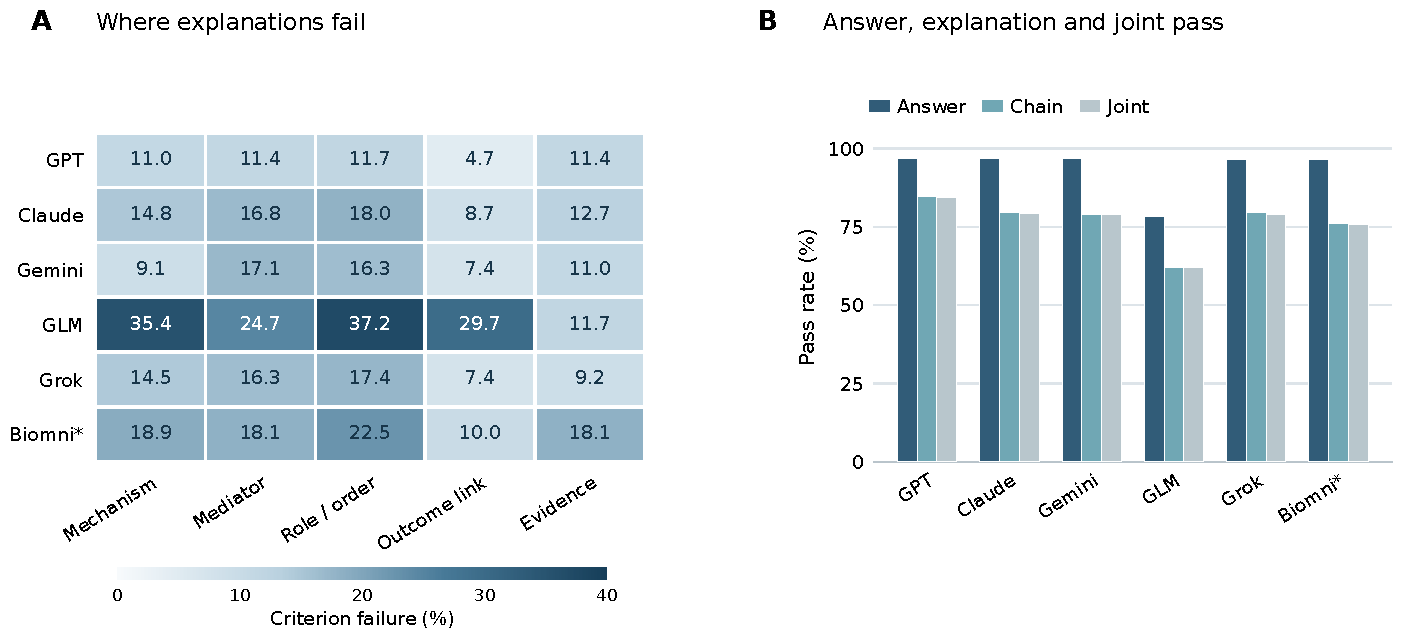
\includegraphics[width=\linewidth]{figs/diagnostic_landscape.pdf}
\caption{Task 2 diagnostics, with 772 unit-run records per system. (A) Failure rates on the five explanation criteria. (B) Answer = correct response direction; Chain = all five criteria pass; Joint = both answer and chain pass. Biomni (*) uses tools; the other systems are closed-book. Abbreviations identify the same systems as Table~\ref{tab:model_performance}.}
\label{fig:s_diagnostics}
\end{figure}
\begin{center}
\begin{tabular}{lrrr}
\toprule
Direction / explanation & Chain pass & Chain fail & Total \\
\midrule
Correct direction & 3,544 & 792 & 4,336 \\
Wrong direction & 14 & 282 & 296 \\
Total & 3,558 & 1,074 & 4,632 \\
\bottomrule
\end{tabular}
\end{center}
Of 1,074 chain-failing records, 792 (73.7\%) predict the correct direction. They represent 17.1\% of all 4,632 Task 2 records. The joint criterion fails on 1,088 records (23.5\%), including the 14 with a wrong direction field despite a passing chain judgment. Those 14 require adjudication review, not a claim that inconsistent answers are mechanistically valid.

Conditioning on accepted answers gives a different denominator: the proportion whose explanations fail ranges from 12.9\% to 21.5\% across systems in Task 2, and from 10.4\% to 54.8\% in Task 3. These are descriptive rates under the existing judges; they are not estimates of population-wide biological reasoning ability.
\begin{center}
\begin{tabular}{lrr}
\toprule
System & T2 fail / correct & T3 fail / correct \\
\midrule
GPT & 96/746 & 9/56 \\
Claude & 136/748 & 8/36 \\
Gemini & 139/748 & 6/51 \\
GLM & 127/605 & 10/51 \\
Grok & 134/744 & 5/48 \\
Biomni & 160/745 & 40/73 \\
\bottomrule
\end{tabular}
\end{center}

\clearpage
\section{Mechanism strata and intervention-specific contrasts}\label{app:strata}
Each mechanism row pools six systems and four runs. ``Med+ / Role-'' counts records passing mediator correctness but failing causal role/order. A pair can contribute multiple intervention units, and the classes differ in input specificity and biological sampling. These summaries do not establish a causal effect of regulatory architecture on model performance.
\begin{center}
\begin{tabular}{lrrrr}
\toprule
Task / mechanism & Pairs & Units & Chain fail / N & Med+ / Role- \\
\midrule
2 / Chromatin & 20 & 20 & 180/480 & 79 \\
2 / Combinatorial & 16 & 35 & 507/840 & 67 \\
2 / RNA & 20 & 26 & 236/624 & 32 \\
2 / Direct cis & 112 & 112 & 151/2688 & 29 \\
3 / RNA & 5 & 10 & 24/240 & 10 \\
3 / Combinatorial & 4 & 10 & 165/240 & 36 \\
\bottomrule
\end{tabular}
\end{center}
\begin{figure}[H]
\centering
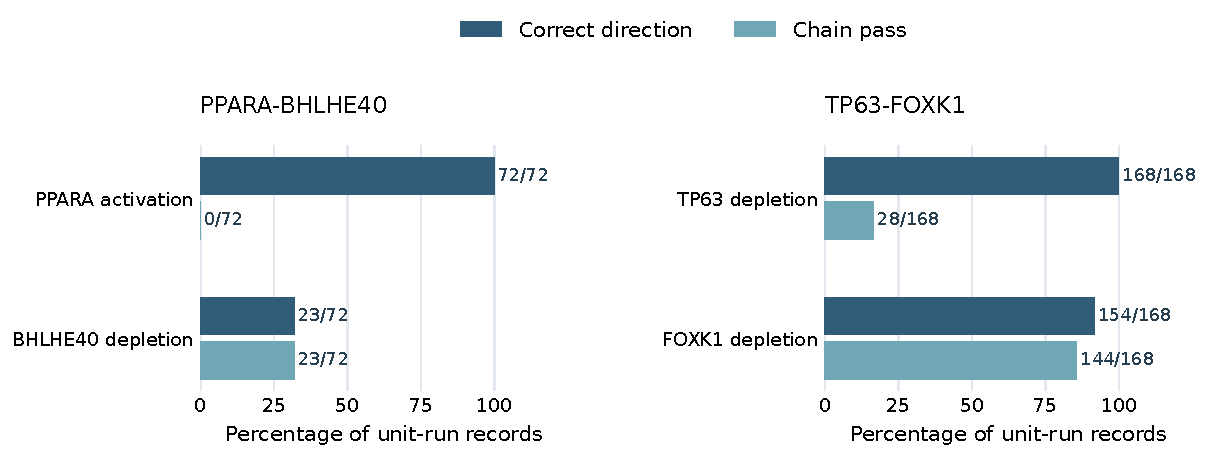
\includegraphics[width=\linewidth]{figs/intervention_contrasts.pdf}
\caption{Descriptive intervention contrasts within two dependency modules. Each bar is labeled with its exact numerator and denominator. Both the supplied entity and the intervention change between the two rows of a module. These are not controlled tests of mediator disclosure.}
\label{fig:s_interventions}
\end{figure}
The PPARA activation subset has 72/72 correct directions and 0/72 chain passes; BHLHE40 depletion has 23/72 for both. TP63 depletion gives 28/168 chain passes, whereas FOXK1 depletion gives 144/168. The same TF--target relationships can therefore show different reconstruction performance under different intervention queries. A controlled disclosure experiment would hold the biology and intervention fixed while varying the information supplied; that experiment has not been performed here.

\clearpage
\section{Cooperative dependencies: PPARA--BHLHE40 and TP63--FOXK1}\label{app:modules}
\subsection{PPARA--BHLHE40: a hepatic regulatory dependency}
The original hepatocyte experiments show that WY-14643 induces Angptl4, Hmgcs2 and Pdk4, and BHLHE40 depletion attenuates this induction~\cite{kokki2026bhlhe40}. This supports a positive functional dependency in the assayed setting; it does not establish that BHLHE40 is a universal coactivator, that it is sufficient for every target, or that a specific direct protein-binding mechanism was proved for each locus.

The PPARA-activation subset (T2U\_0036--0038) contains 72/72 correct direction predictions and 0/72 complete-chain passes. BHLHE40 is named in only three responses, all from GPT run 4, which instead describe it as opposing the regulatory program. The BHLHE40-depletion subset (T2U\_0039--0041) has 23/72 correct direction predictions and 23/72 chain passes; the other 49 predict the wrong direction. Pooling both subsets gives 121/144 chain failures. The distinction is biologically informative: a familiar receptor-activation endpoint is recovered without its curated partner dependency, whereas directly intervening on that partner exposes errors in its functional sign. Intervention identity, direction and input entity all differ, precluding an isolated mediator-disclosure effect.

In Task 3, T3VP\_0002 supplies BHLHE40 and a decrease in Pdk4. Fifteen responses canonically predict overexpression, eight predict knockdown and one embeds the entity in a nonaccepted type string. For T3VP\_0004, 17/24 canonically predict overexpression, six agonist activation and one a nonaccepted entity-bearing string. Biomni supplies an accepted agonist type in all four runs but passes the chain in none. These are separate examples of intervention-method agreement and dependency recovery. Neither decreased expression nor receptor activation alone uniquely identifies the experimental method.

\subsection{TP63--FOXK1: cooperation with a spatial regulatory function}
The source work links the p63--FOXK1 partnership to carcinoma-specific chromatin loops and transcription of associated targets~\cite{jung2026foxk1}. FOXK1 therefore represents a biologically grounded dependency with a spatial regulatory function, rather than an arbitrary extra name in the answer key. The seven targets are selected experimentally from a shared regulatory program; they are not seven independent demonstrations across tissue lineages.

On the seven TP63-depletion units, GPT names FOXK1 in 21/28 responses and Gemini in 7/28; those responses pass the complete chain. Claude, GLM, Grok and Biomni name FOXK1 in 0/112 combined responses and contribute no chain passes on this subset. In the seven FOXK1-depletion units, the same four systems produce 88/112 chain passes, and all six systems together produce 144/168. Thus ``four systems never name FOXK1'' holds only for the TP63-depletion subset. It does not hold for the complete 14-unit module. This contrast supports testing dependency retrieval separately from application of a supplied dependency.

\paragraph{Development implication.} These modules motivate distinguishing retrieval of an omitted partner from application of a supplied partner. Training examples could preserve the same experimentally supported dependency while querying different intervention entry points. The contrasts above suggest this evaluation design; they do not show that supplying a mediator is itself the cause of better performance.

\clearpage
\section{Regulatory process and sign: GATA1 and SRCAP/H2A.Z}\label{app:function}
\subsection{GATA1--TAL1/LMO2: occupancy versus productive recruitment}
In the erythroid complementation experiments, D218G/R216Q impair recruitment of the TAL1 complex through the LMO2-associated interaction while GATA1 occupancy is largely retained; FOG1 recruitment is not equivalently lost~\cite{campbell2013gata1}. Describing this simply as disruption of a direct GATA1--TAL1 interface would overstate the molecular resolution. The functional lesson is that binding and productive cofactor recruitment can be separable regulatory steps.

Across six units (three targets and two variants), 142/144 directions are correct but 14/144 chains pass: six from Grok run 1 and eight distributed across Biomni runs. The six Grok explanations describe a defective partner interaction without explicitly naming TAL1. We retain their archived judgments and flag their mediator-specificity for review. A passing automated score cannot be treated as proof that the exact complex was recovered. Conversely, a biologically plausible FOG1 explanation is insufficient when the experiment implicates a different retained-versus-disrupted interaction. The proposed training target is variant-specific process identification, not generic classification of a mutation as loss of function.

\subsection{SRCAP/H2A.Z: a context-specific regulatory sign}
The original H226 squamous carcinoma study supports repression of anti-proliferative genes through $\Delta$Np63$\alpha$-associated SRCAP machinery and H2A.Z; SAMD9L depletion rescues the proliferation arrest after p63 depletion~\cite{gallant2012deltanp63alpha}. This connects the sign of regulation to a functional experimental phenotype. H2A.Z should not be assigned a universal activating or repressive role across contexts.

Across two units, 44/48 judgments fail causal role/order and 46/48 fail the full chain. Thirty-six pass mediator correctness but fail causal role/order. For SAMD9L alone (T2U\_0022), 23/24 predict the wrong direction and 23/24 fail the chain; 22/24 fail the causal-role axis. These denominators differ because the five axes are scored separately. This is a specific diagnostic for sign assignment conditional on a recognized component, not a claim of a general inability to reason about chromatin.

\begin{center}
\begin{tabular}{ll}
\toprule
Diagnostic & Numerator / denominator \\
\midrule
GATA1 correct direction & 142/144 \\
GATA1 complete chain & 14/144 \\
Grok chain passes without explicit TAL1 & 6/6 Grok passes \\
H2A.Z mediator pass but role fail & 36/48 \\
SAMD9L wrong direction & 23/24 \\
\bottomrule
\end{tabular}
\end{center}
The two modules distinguish different evaluation targets. In the variant case, a generic loss-of-function explanation can name a plausible cofactor yet miss the affected molecular step. In the chromatin case, the mediator can be recognized but assigned the wrong sign. A training or evaluation objective that rewards only molecular names cannot distinguish these errors. The GATA1 mediator-specificity flags also show why process-level and exact-complex correctness should be reported separately.

\clearpage
\section{Input ambiguity and sensitivity analyses}\label{app:sensitivity}
\subsection{ESR1 enhancer interference}
The source uses SID4X--dCas9--KRAB enhancer interference in estradiol-responsive Ishikawa cells. HDAC-dependent enhancer deactivation, reduced H3K27ac, and rescue with an HDAC inhibitor support an epigenetic dependency~\cite{carleton2017enhancer}. This differs from assuming that the regulatory DNA was physically deleted. It is also a case in which cis-element function and chromatin mediation are biologically connected despite different benchmark labels.

All 72 direction predictions are correct, while 70/72 causal-role and 71/72 chain judgments fail. Biomni contributes the single chain pass (CISH, run 1) and the additional causal-role pass (MMP17, run 3). The model inputs omit the specific interference method. Consequently, this module motivates richer intervention descriptions and the sensitivity analysis below; it should not be presented as unqualified evidence of a model knowledge deficit.

Three ESR1 units (T2U\_0013--0015) describe loss/reduction of target regulatory sites, while evaluator-side records specify epigenetic repression. A direct-cis site-loss reading is therefore defensible. The table excludes these three units without altering any score on the remaining 190 units. It also reports pair weighting on the original 193 units: average judgments within each pair, then average equally over the 168 pairs. Pair weighting addresses unit multiplicity, not shared-source dependence.
\begin{center}
\begin{tabular}{lrrr}
\toprule
System & Original chain & No ESR1 & Pair-weighted \\
\midrule
GPT & 84.7 & 86.1 & 86.9 \\
Claude & 79.4 & 80.7 & 83.9 \\
Gemini & 79.0 & 80.3 & 82.2 \\
GLM & 62.0 & 63.0 & 66.3 \\
Grok & 79.5 & 80.8 & 82.9 \\
Biomni & 76.2 & 77.2 & 80.1 \\
\bottomrule
\end{tabular}
\end{center}
No new source-study cluster confidence interval is claimed: multiple targets can share a study or regulatory module, and pair weighting does not remove that dependence. This appendix deliberately reports descriptive sensitivities instead of treating repeated runs as biological replication.


\paragraph{Interpretation of sensitivity.} Excluding the three ESR1 units increases every system's Task 2 chain rate while preserving their ordering. Pair weighting also changes the absolute rates because a repeated pair no longer contributes more total weight solely through multiple units. Neither operation corrects judge error or shared-source dependence. The original primary values are retained, and these alternatives are reported transparently rather than selected as replacement headline results.

\clearpage
\section{Shared failures and inverse intervention ambiguity}\label{app:shared_failures}
A strict shared-failure unit has no chain pass in any of the six systems' four runs (24/24 failures). A strict shared-failure pair requires that property for every intervention unit associated with the pair within the task. This is stronger than failure in the first run or failure on one selected intervention. Neither definition establishes universal inability outside the tested inputs.

\begin{center}
\begin{tabular}{llrrr}
\toprule
Task & Unit(s) & Mechanism fail & Mediator fail & Role fail \\
\midrule
2 & T2U\_0014 (ESR1--G0S2) & 24/24 & 24/24 & 24/24 \\
2 & T2U\_0015 (ESR1--MMP17) & 23/24 & 23/24 & 23/24 \\
2 & T2U\_0036--0038 (PPARA targets) & 66/72 & 69/72 & 69/72 \\
3 & T3VP\_0004, 0005, 0012 (PPARA) & 70/72 & 70/72 & 72/72 \\
\bottomrule
\end{tabular}
\end{center}
There are five strict shared-failure units in Task 2 and three in Task 3. Only two Task 2 pairs fail on every available intervention unit: ESR1--G0S2 and ESR1--MMP17, both subject to the query ambiguity described above. No Task 3 pair fails on all its intervention units. The three PPARA targets are shared failures under receptor activation in both tasks, but other interventions on those pairs can pass. The inference is therefore intervention-dependent failure to recover a curated dependency, not a universally unresolvable pair.

\paragraph{Three inverse-inference distinctions.} An accepted intervention label identifies agreement with the curated experiment. A compatible alternative may yield the same response without being the method used in that experiment. A wrong molecular role can instead generate a different explanation whose apparent directional consistency depends on that role inversion. These three situations must not be collapsed into a single claim of missing biological knowledge.
\begin{center}
\begin{tabularx}{\linewidth}{@{}p{.17\linewidth}XX@{}}
\toprule
Example & Curated intervention & Interpretation \\
\midrule
T3VP\_0002 & BHLHE40 siRNA knockdown & 15 canonical overexpression answers; inversion of BHLHE40's role can make an alternative story appear direction-consistent. \\
T3VP\_0004 & PPARA agonist activation & 17 canonical overexpression answers; endpoint direction does not uniquely recover the method. Biomni's 4/4 accepted labels coexist with 0/4 chain passes. \\
T3VP\_0009 & Combined pathway stimulation & Generic activation need not recover the specified combined operation; method specificity and pathway reasoning are separate properties. \\
\bottomrule
\end{tabularx}
\end{center}

\clearpage
\section{Prediction concentration and adjudication sensitivity}\label{app:concentration}
The following confusion summary uses the schema-compliant released Task 1 runs, including the re-administered GLM run retained in the frozen release. It does not mix the archived schema-deviant capture into the denominator.
\begin{center}
\begin{tabular}{lrrr}
\toprule
Gold class & Predictions & Direct-cis predictions & Correct class \\
\midrule
Direct cis & 2,736 & 2,585 (94.5\%) & 2,585 (94.5\%) \\
Chromatin & 504 & 418 (82.9\%) & 43 (8.5\%) \\
Combinatorial & 384 & 340 (88.5\%) & 40 (10.4\%) \\
RNA & 480 & 400 (83.3\%) & 51 (10.6\%) \\
\bottomrule
\end{tabular}
\end{center}
Direct cis accounts for 3,743/4,104 predictions (91.2\%), compared with 114/171 reference pairs (66.7\%). This is evidence of concentrated predictions under the present inputs. Identical prompts do not exclude prompt effects; symmetric class scoring does not eliminate effects of imbalance, omitted context or the annotation ontology. No architectural cause is established by this confusion summary.

The Task 2 direction/chain cross-tabulation is: direction correct and chain pass, 3,544; direction correct and chain fail, 792; direction wrong and chain fail, 282; direction wrong and chain pass, 14. These sum to 4,632. The last group and the six generic-partner GATA1 passes are identified for targeted human adjudication. They remain unchanged in all primary tables. Across systems, units failing exactly one axis in at least one run number 12 (GPT), 6 (Claude), 32 (Gemini), 0 (GLM), 5 (Grok) and 4 (Biomni); these overlapping per-system sets are not new independent samples.

\begin{center}
\begin{tabular}{lrrr}
\toprule
System & NANOG--Nanog & POU5F1--Pax6 & Total flagged \\
\midrule
GPT & 3 & 1 & 4 \\
Claude & 1 & 0 & 1 \\
Gemini & 1 & 0 & 1 \\
GLM & 1 & 0 & 1 \\
Grok & 2 & 0 & 4 \\
Biomni & 1 & 0 & 3 \\
\bottomrule
\end{tabular}
\end{center}
\paragraph{Format sensitivity.} GLM Task 2 runs 3 and 4 contain 51 and 98 exact copies of the input intervention class in the direction field; run 3 additionally contains one blank direction. These outputs remain scored as submitted. An interpretable but noncanonical Task 3 method string is likewise distinct from a biologically contradicted mechanism. Format-aware secondary analyses should be disclosed as alternatives, not substituted silently into frozen primary scores.

\clearpage
\section{Training hypotheses and reproducibility of diagnostic claims}\label{app:training}
The benchmark motivates the following research designs; none is a training result of this study.
\begin{center}
\begin{tabularx}{\linewidth}{@{}p{0.18\linewidth}XX@{}}
\toprule
Observed diagnostic & Candidate supervision & Evidence needed to show improvement \\
\midrule
Partner omission & Required dependency and mediator identity, paired across intervention entry points & Improvement on source- and pair-disjoint modules when the mediator is withheld, alongside performance when supplied \\
Wrong role despite mediator pass & Context-conditioned signed causal relations and intervention--outcome consistency & Better role accuracy without sacrificing entity accuracy; external evidence checks beyond internal graph consistency \\
Generic variant explanation & The experimentally affected step: occupancy, recruitment or downstream transcription & Generalization to held-out variants with distinct molecular effects; exact-complex and process-level scores reported separately \\
Method ambiguity & Compatible intervention sets, evidence-conditioned method inference and calibrated uncertainty & Distinguish acceptance of biologically compatible alternatives from recovery of the actual source experiment \\
\bottomrule
\end{tabularx}
\end{center}
The key development objective is preserving an experimentally grounded dependency under changes in the queried intervention, rather than rewarding a plausible narrative or a molecular-name list. A future controlled comparison would hold biological context and the perturbation fixed while varying mediator disclosure or supporting evidence. It would also separate answer formatting from biological content and use independently adjudicated held-out references. Such designs can test the hypotheses suggested by the present natural contrasts without attributing those contrasts prematurely to a single cognitive or architectural cause.
\paragraph{A worked diagnostic trace.} For T2U\_0036, the model input supplies PPARA, Angptl4 and PPARA gain/activation; the evaluator-side record requires the BHLHE40-associated dependency. All 24 responses predict up, but none passes the chain. This unit contributes to an outcome--mechanism dissociation rather than an endpoint error. The archived prediction, mediator annotation and five axis values can be inspected separately; the module scripts export the complete rows instead of only an aggregate rate.

\paragraph{Portable reproduction.} The accompanying reviewed repository provides \path{scripts/reproduce_release.py} for archived-record checks and main-table recomputation, and \path{scripts/analyze_dependency_modules.py} for the module contrasts and strict shared-failure lists. Frozen predictions and judgments remain unchanged. The original manifest is retained separately from the revised-package manifest. A third party can therefore inspect the same examples, reproduce the reported denominators and identify which judgments would change under a new adjudication protocol.
